\documentclass[ignoreonframetext,unicode]{beamer}

\usepackage[utf8]{inputenc}
\usepackage[T1]{fontenc}
\usepackage[english,russian]{babel}
\usepackage{amsmath}
\usepackage{amsfonts}
\usepackage{amssymb}
\usepackage{graphicx,pgf}
\usepackage{multimedia}

\usetheme{Warsaw}

\useinnertheme{circles}   %внутренняя тема
%\useoutertheme{smoothbars}   %внешняя тема
\usecolortheme{seahorse}     %цветовая схема
%\usefonttheme{serif}    %шрифты
%\defbeamertemplate*{footline}{shadow theme}
%\setbeameroption{hide notes}

\graphicspath{{./style/}{./figures/}}

%номера слайдов
\newcommand*\oldmacro{}%
\let\oldmacro\insertshorttitle%
\renewcommand*\insertshorttitle{%
	\oldmacro\hfill%
	\insertframenumber\,/\,\inserttotalframenumber}
\RequirePackage{caption}
\DeclareCaptionLabelSeparator{defffis}{ }
\captionsetup{justification=centering,labelsep=defffis}

%\title{Курсовая работа}
%\subtitle{Численные схемы для аппроксимации неограниченных решений при моделировании обтекания профиля крыла в вихревых методах}
\title[Кручение стержня]{Кручение стержня\\ прямоугольного сечения}
\author[Пиневич В.\,Г.]{Докладчик: Пиневич В.\,Г.\and\\[0.5mm] Научный руководитель: Котович А.\,В.}

\institute[каф. Прикладная математика ФН-2]{группа ФН2-51Б}
\date{\today}
\titlegraphic{
\includegraphics[width=2cm]{logo.png}}
%\renewcommand{\vec}[1]{\text{\mathversion{bold}${#1}$}}


\begin{document}
	
	\begin{frame}[plain]
		\maketitle
		%\insertshortinstitute{Группа ФН2-41Б}
	\end{frame}

	\begin{frame}{Постановка задачи}
		\begin{columns}
			\column{\textwidth}`
			\begin{block}{Функция кручения}
			 \[
	\label{funCruc}
\Delta \psi = \frac{\partial^2 \psi }{\partial x^2} +
\frac{\partial^2 \psi }{\partial y^2} = -2G \theta 
			 \]
			\end{block}

		\begin{columns}
			\column{0.5\textwidth}
			Сравнить два решения задачи о кручении стержня прямоугольного сечения, полученных энергетическим методом и методом Ритца. Выяснить зависимости точности решения в обоих случаях от числа членов ряда и сравнить полученные результаты
			\column{0.5\textwidth}
			\includegraphics[width=\textwidth]{sterzhenСruchenie}
		\end{columns}

		\end{columns}
		
	\end{frame}

	\begin{frame}{Энергетический метод}	
		
		\begin{columns}
			\column{0.5\textwidth}
			\begin{block}{Требуется решить уравнение}	
				\[
Au = f, f \in H
				\]
			\end{block}
		\column{0.5\textwidth}
		\begin{block}{Энергетическое произведение}	
\[
[u, v] = (Au, v)
\]
		\end{block}
		\end{columns}
				
	\begin{columns}
		\column{0.5\textwidth}
		\begin{block}{Решение сводится к поиску минимума функционала}	
	\[
	F(u) = (Au, u) - 2(u, f)
	\]
\end{block}
			\column{0.5\textwidth}
	\begin{block}{Решение можно представить в виде}
		\[
		u_0 = \sum\limits_{n = 1}^{\infty} (f, \omega_n)\omega_n
		\]
	\end{block}
	\end{columns}
	
	\end{frame}

\begin{frame}{Метод Ритца}
	\begin{block}{Линейная комбинация первых $n$ координатных элементов}	
	\[
	u_n = \sum_{i = 1}^n a_i \, \varphi_i
	\]
\end{block}
		
	\begin{block}{Для вычисления коэффициентов $a_i$}	
		\[
		F = - \int\limits_0^a \int\limits_0^b \left(
		\frac{1}{2}
		\left(\frac{\partial\psi}{\partial x}\right)^2 + 
		\frac{1}{2}
		\left(\frac{\partial\psi}{\partial y}\right)^2
		-2G\theta\psi
		\right) dx dy
		\]
	\end{block}

\begin{block}{Для получения минимума $F$}
	\[
		\frac{\partial F(u_n)}{\partial a_i} = 0, \qquad i = 1, 2, \ldots, n
	\]
\end{block}
	
\end{frame}	

\begin{frame}{Задача}
	
		\begin{block}{Условие}
		Рассмотрим задачу о кручении стержня, основание которого представляет собой   прямоугольник
		$0 \leqslant x \leqslant a$, $0 \leqslant y \leqslant b$.
	\end{block}
		\begin{block}{}
		Функция кручения $\psi(x, y)$ удовлетворяет условию $-\Delta \psi = 2 G \theta$.
	\end{block}
\begin{block}{}
		Функция $\psi(x, y)$ обращается в нуль на
		сторонах прямоугольника $x= 0$, $x = a$, $y = 0$, $y = b$.
		\end{block}
	
\end{frame}

\begin{frame}{Решение энергетическим методом}
	\begin{block}{Функция кручения}	
		\[
		\psi(x, y) = \sum_{m, n = 1}^\infty (2G \theta, \psi_{mn}) \, \psi_{mn}(x, y)
		\]
	\end{block}
		\begin{block}{}
	\[
	(2G \theta, \psi_{mn}) = \frac{4 G \theta}{\pi}\int\limits_0^a \sin\left(\frac{m \pi x}{a}\right) dx \int\limits_0^b
	\sin\left(\frac{n \pi y}{b}\right) dy = 
	\]
	\[
	= \frac{4abG\theta}{\pi^3 mn} \sqrt{\frac{ab}{b^2 m^2 + a^2 n^2}}
	\]
\end{block}
\begin{block}{Итоговое выражение}	
	\[
	\psi(x, y) = \frac{32 a^2 b^2 G\theta}{\pi^4} \!\!\! \sum_{m, n = 1, 3, 5, \ldots}
	\!\!\! \frac{\sin\dfrac{m\pi x}{a} \, \sin\dfrac{n\pi y}{b}}{mn(b^2 m^2 + a^2 n^2)}
	\]
\end{block}
\end{frame}

\begin{frame}{}
	\begin{block}{Значения функции кручения в середине прямоугольника}	
	\[
		\begin{aligned}[b]
		\psi\left(\frac{1}{2}, \frac{1}{2}\right) = 0.144G\theta\mbox{, при } n, m = 1, 3, \\
		\psi\left(\frac{1}{2}, \frac{1}{2}\right) = 0.147G\theta\mbox{, при } n, m = 1, 3, \ldots21,\\
		\psi\left(\frac{1}{2}, \frac{1}{2}\right) = 0.147G\theta\mbox{, при } n, m = 1, 3, \ldots209.
	\end{aligned}
	\]
	\end{block}

	\begin{columns}
	\column{0.5\textwidth}
	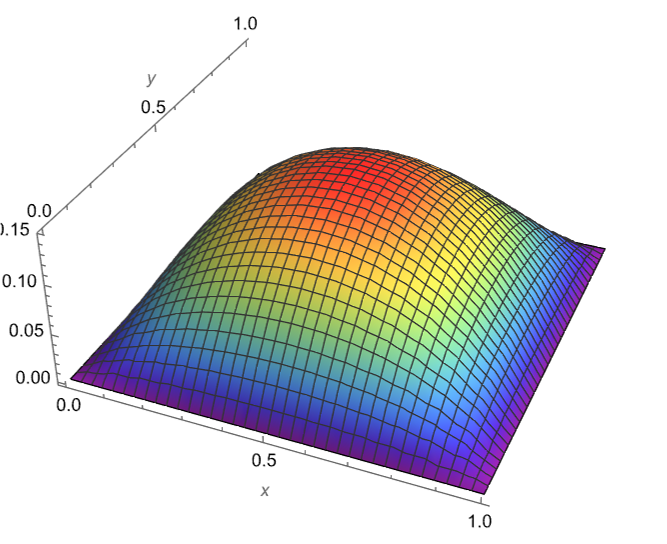
\includegraphics[width=\textwidth]{ser_graph}%
	\column{0.4\textwidth}
	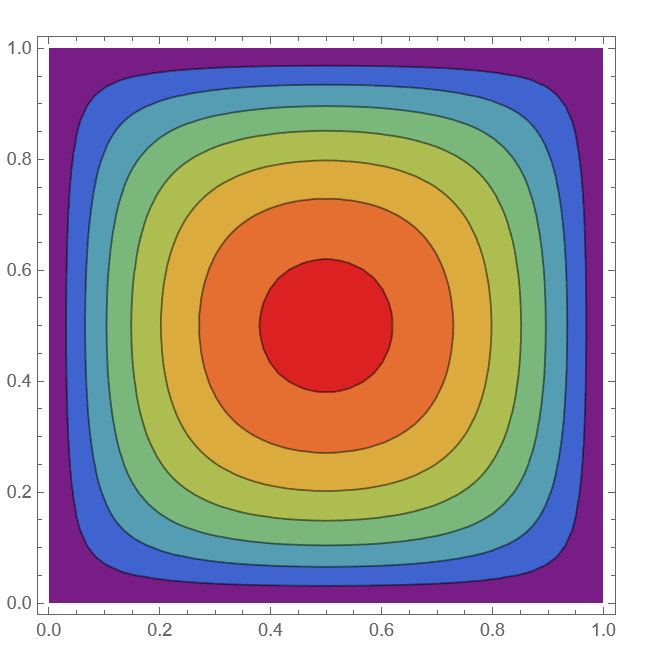
\includegraphics[width=\textwidth]{ser_levels}%
\end{columns}
\end{frame}

\begin{frame}{Решение методом Ритца}
		\begin{block}{Полагая для упрощения $\psi = 2G \theta u$, получим задачу в виде}	
\[
\begin{cases}
	-\Delta u = 1, \\
	\psi(a, y) =  \psi(x,b) = 0, \\
	\psi(0, y) =  \psi(x,0) = 0.
\end{cases}
\]
	\end{block}

\begin{block}{}	
\[
\psi(x, y) = x(x - a)y(y - b)\left(a_0 + a_1\left(x + y\right) + a_2\left(x^2 + a_3 y^2\right) + \ldots\right)
\]
\end{block}

	\begin{block}{Первый порядок точности}	
		\[
			\psi_1(x, y) = a_0 x(x - a)y(y - b)
		\]
	\end{block}

	\begin{block}{Второй порядок точности}	
	\[
		\psi_2(x, y) = x(x - a)y(y - b)\left(a_0 + a_1\left(x + y\right) + a_2\left(x^2 + a_3 y^2\right)\right)
	\]
\end{block}

\end{frame}

\begin{frame}{}

		\begin{columns}
	\column{0.5\textwidth}
	\begin{block}{Первый порядок точности}	
		\[
			\psi_1\left(\frac{1}{2}, \frac{1}{2}\right) \approx 0.156 G \theta
		\]
	\end{block}
	\column{0.5\textwidth}
	\begin{block}{Второй порядок точности}	
		\[
		\psi_2\left(\frac{1}{2}, \frac{1}{2}\right) \approx 0.146 G \theta
		\]
	\end{block}
\end{columns}

	\begin{columns}
	\column{0.5\textwidth}
	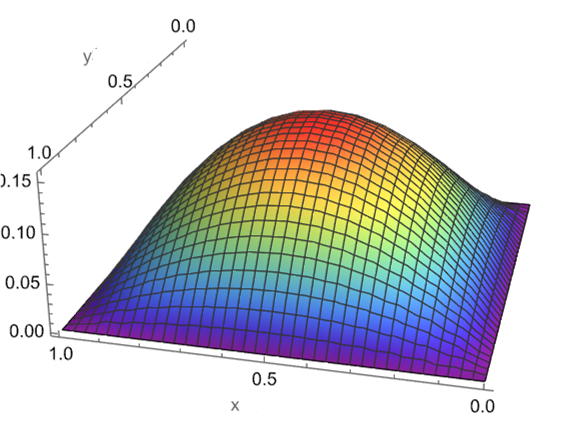
\includegraphics[width=\textwidth]{ritz_graph}%
	\column{0.5\textwidth}
	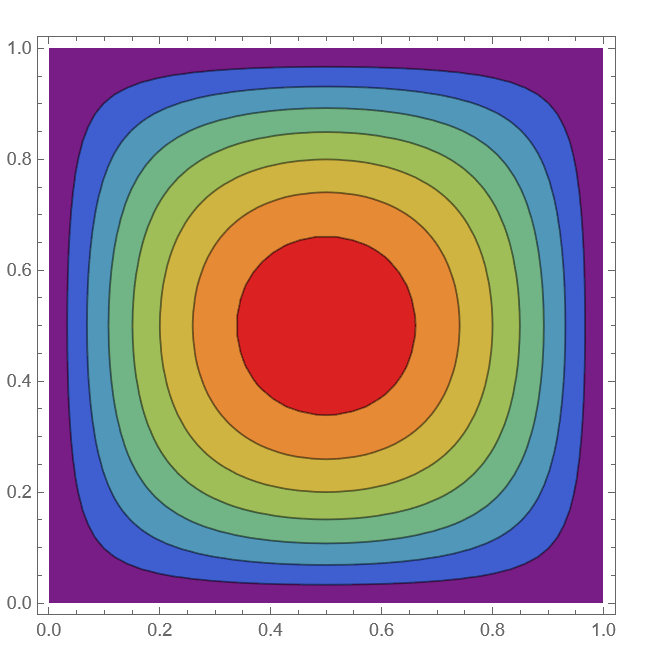
\includegraphics[width=\textwidth]{ritz_levels}%
\end{columns}
\end{frame}

\begin{frame}{Сравнение функций кручения}


\begin{block}{}
	$\psi\left(\frac{1}{2}, \frac{1}{2}\right) = 0.147G\theta$ для энергетического метода и $\psi\left(\frac{1}{2}, \frac{1}{2}\right) = 0.146G\theta$ для метода Ритца, они отличаются на 1\%. При этом при малой точности вычисления данные методы дают результат $0.144G$ и $0.156G$ соответственно. Точным решением является $\psi\left(\frac{1}{2}, \frac{1}{2}\right) = 0.147G\theta$, из чего мы можем сделать вывод, что метод энергий более точный в рассматриваемом случае
\end{block}

\begin{columns}
	\column{1\textwidth}
	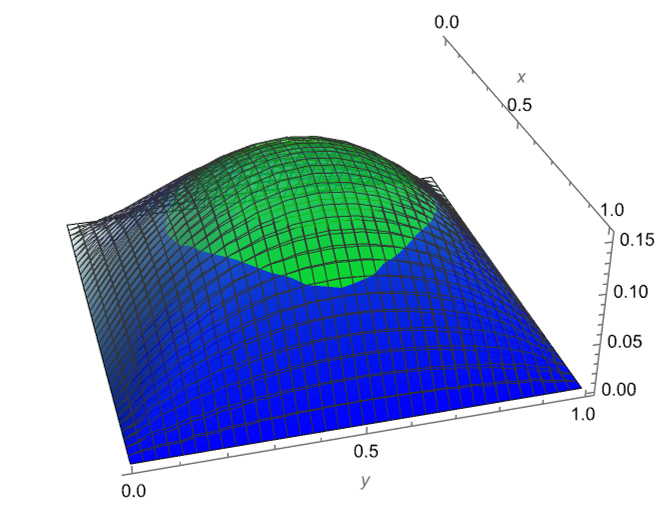
\includegraphics[width=1\textwidth]{compare3d}
\end{columns}
	

\end{frame}

\begin{frame}{Сравнение крутящих моментов}
	
	\begin{block}{Крутящий момент определяется формулой}	
	\[
	M = 2 \int\limits_{-a}^a \int\limits_{-b}^b \varphi dx dy
	\]
	\end{block}	
	
	\begin{block}{Энергетический метод}	
\[
	M_{\text{Э}} = \frac{256 G \theta a^4 b^4} {\pi^6}\!\!\!\sum_{m, n = 1, 3, 5, \ldots}\!\!\!\frac{1}{(b^2 m^2 + a^2 n^2 )m^2 n^2}
	= 0.140G\theta a^4
\]
	\end{block}
\begin{columns}
	\column{0.5\textwidth}
\begin{block}{1-е приближение м. Ритца}
\[
M_{\text{Р}_1} = 0.139(2a)^4
\]
\end{block}
\column{0.5\textwidth}
\begin{block}{2-е приближение м. Ритца}
\[
M_{\text{Р}_2} = 0.140(2a)^4
\]
\end{block}
\end{columns}

\end{frame}

\begin{frame}{Результаты}
	В ходе работы получены следующие результаты:
	\begin{block}{}
	\begin{enumerate}
		\item С помощью рассмотренных методов была решена задача кручения прямоугольного стержня, их результаты оказались идентичны с точностью до второго знака.	
		\item Оба метода позволяют вычислить крутящий момент с точностью до третьего знака.
		\item Энергетический метод позволяет получить ответ  несколько точнее и быстрее, но каждый раз требует вычисления тригонометрического ряда.
		\item 
		Метод Ритца дает возможность получить функцию кручения в виде многочлена и получать ответ с другими параметрами задачи с меньшим количеством вычислений, что может быть полезно при большом объеме вычислений.
	\end{enumerate}
	\end{block}	
\end{frame}	
\end{document} 